\cotefile{10}
\scanpage{69}
% archive sheet number: 68

$E$ sur $K$, munis d'un \deleted{\unsure{endomor}} \uline{automorphisme} $\handwritten{\sigma}$-linéaire $F_E$\handwritten{;} \deleted{\unsure{$E\quad E$}} qu'on a intérêt à interpréter comme un isomorphisme $K$-linéaire
\[
F_E : E^{\handwritten{\sigma}} = E\otimes_K(K,\handwritten{\sigma})\handwritten{\longrightarrow} E\ .
\]
Les opérations tensorielles sont définies par transport de structure (cf. cas d'un groupe, ici $\underline{Z}$, opérant sur un corps ....). Les F-isocristaux effectifs s'interprètent alors comme les $(E,F_E)$ tels que $F_E$ laisse invariant un réseau, ce qui signifie aussi que l'ensemble des itérés $F_E^n$, $n\handwritten{\geq}0$, est \uline{borné} dans \unsure{l'e|le}\deleted{\unsure{x}} vectoriel $\operatorname{End}(E)$. Tout$(E,F_E\unsure{)}$ devient \inserted{évidemment} effectif après multiplication de $F_E$ par une puissance convenable de $p$, ce qui est une autre façon de dire que la catégorie des F-iso\unsure{c|w}ristaux se déduit de celle des F-\deleted{\unsure{si}}\handwritten{\unsure{is|si}}ocristaux effectifs \deleted{par} en rendant \unsure{inversible|ènversible} $K\handwritten{(}-1)$ .

\handwritten{4.} La catégorie tannakienne $\mathrm{Fcriso}(k)$ est un invariant arith\inserted{\handwritten{m}}étique intéressant attaché à $k$ (fonctoriellement); sa \deleted{donnée} connaissance équivaut à celle de la gerbe associée (sur $\underline{Q}_p$), soit $\underline{G}(k)$\handwritten{\unsure{.|;}} Parmi les structures supplémentaires qu'il convient d'étudier en même temps que cette gerbe, il faut inclure la structure d'effectivité de la catégorie $\mathrm{Fc}\handwritten{\mathrm{ri}}\mathrm{so}(k)$ de\deleted{s} ses représentations linéaires, celle de l\deleted{\unsure{à|a}}\handwritten{'}objet de \deleted{\unsure{F}}\handwritten{T}ate inverse (définissant un homomorphisme canonique de $\underline{G}(k)$ vers la gerbe triviale de groupe $\underline{G}_m$), enfin pour $k$ parfait tout au moins, la donnée du foncteur fibre naturel sur $K(k)$ (qui est donc une section de la gerbe $\underline{G}(k)$ sur $K(k)$); pour $k$ non parfait, il con\deleted{\unsure{nai}}viendrait \deleted{de} d'étudier de même la section de $\underline{\unsure{G|E}}(k)$ sur le corps des fractions $K$ de n'importe quel $p$-anneau $W$ de corps résiduel $k$.

L'intérêt de la notion de F-cristal \deleted{non dégénéré} provient du fait que l'on \deleted{\unsure{n}}\unsure{a|â} un foncteur ``cohomologie cristalline''
\[
X\handwritten{\unsure{\longmapsto|\mapstochar\relbar}} H^{\handwritten{*}\deleted{\unsure{k|i}}}_{\mathrm{cris}}(X)
\]

\scanpage{70}
% archive sheet number: 69

allant de la catégorie des schémas propres et lisses sur $k$ vers les F-cristaux gradués, \deleted{compatibles} qui est additif (pour la somme des $X$ ) et compatible avec $\otimes$ \inserted{\handwritten{une fois tensorisé par $\mathbb{Q}_p$}} (le $\otimes$ des schémas étant le produit cartésien) de façon compatible avec les associativités et commutativités (tant pour la somme que pour le produit), en faisant attention d'utiliser la règle de Koko pour la contrainte de commutativité. De plus, modulo des vérifications qui n'ont pas encore été faites par Berthelot, mais qui ne peuvent manquer de sortir prochainement, le foncteur précédent est même défini en prenant comme morphismes des correspondances algébriques à équivalence algébrique près, et s'en va vers les F-cristaux \uline{non dégénérés}; de façon précise, il doit être vrai que pour tout $i$, il existe un $V_i$ :\deleted{dans} $H^i\handwritten{\longrightarrow (}H^i\handwritten{)^{\sigma}}$ tel que $F\ V_i=p^i\ \mathrm{id}$ , $V_iF=p^i\ \mathrm{id}$ (C'est en tous cas vrai si $X$ se remonte en car. 0) Modulo cette vérification, on trouve donc un foncteur
\[
H^{\handwritten{*}}_{\mathrm{cris}}\deleted{\unsure{\mathbb{W}}}\handwritten{\unsure{\otimes}\mathbb{Q}_p}:\text{schémas propres lisses sur }k\handwritten{\longrightarrow \mathrm{Grad}^{\unsure{\sim}}(}\mathrm{F}\unsure{\mathbb{C}|\mathrm{C}|\mathrm{c}}\mathrm{riso}^{\handwritten{+}}(k)\handwritten{)}\ ,
\]
compatible à\deleted{\unsure{,}} tout (un ``foncteur cohomologie\deleted{\unsure{que}}'' dans la terminologie de l'exposé de Kleiman \handwritten{[\quad]}). Bien entendu, on a $H^{\handwritten{2}}_{\mathrm{cris}}(P^1)=\mathbb{W}(-1)$ , plus généralement on devra avoir (quand Berthelot aura bien travaill\unsure{é)}
\[
H^{2d\deleted{\unsure{*}}}_{\mathrm{cris}}(X)\handwritten{\simeq}\mathbb{W}(-d)
\]
si $X$ est géométriquement connexe et de dimension $d$, (isomorphisme canonique, compatible à la multiplication ...). En admettant le yog\unsure{a} des motifs (on a besoin ici de la structure graduée de la catégorie des motifs sur $k$, pour pouvoir canuler par la règle de Koko la contrainte de commutativité naturelle sur les motifs, provenant de l'isomorphisme de commutativité $X\mathrm{x}Y\handwritten{\simeq}Y\mathrm{x}X$ sur les schémas ...) on aura un homomorphisme de gerbes canonique
\[
\handwritten{\Pi}(k)_{\handwritten{\mathbb{Q}_p}}\handwritten{\longleftarrow}\underline{G}(k)\ ,\qquad
\handwritten{\text{associé au }\inserted{\text{$\otimes$-foncteur}}\mathrm{Mot}(k)\longrightarrow\mathrm{Fcriso}(k)}
\]
où $\handwritten{\Pi}(k)$ est la gerbe associée à la catégorie tannakienne (sur $\underline{Q}$)

\scanpage{71}
% archive sheet number: 70

des \inserted{(iso)}motifs \inserted{(semi-simples)} sur $k$, et l'indice $\underline{Q}_p$ désigne le \deleted{effet du} changement de base par $\underline{Q}\handwritten{\longrightarrow}\underline{Q}_p$ . Cet homomorphisme est compatible à l'augmentation ``de Tate'' et aux structures d'effectivité. Modulo du travail à faire de Berthelo\handwritten{t}, pour $k=\handwritten{\mathbb{F}}_q$ un corps fini à $q$ éléments, la connaissance de l'image \deleted{de $X$ dans} $H^*(X)$ dans $\mathrm{Fcriso}(k)$ permet de calculer \unsure{la|sa} fonction $\handwritten{\zeta_X}$ de $X$, par la formule qu'on devine et que je me dispose \unsure{décrire|d'écrire}. (D'ailleurs, modulo les conjectures de Weil, la connaissance de la fonction $\handwritten{\zeta_X}$ permet, grâce à cette formule, de réconstituer $H^{\handwritten{*}}_{\mathrm{cris}}(X)$ à isomorphisme près dans $\mathrm{Fcriso}(k)$, du moins virtuellement (i.e. l'image de chaque $H^i_{\mathrm{cris}}(X)$ dans l'anneau $K(\mathrm{Fcriso}(k)))$ si on ne désire pas admettre que \deleted{\unsure{tous}} les $H^i$ sont nécessairement des éléments semi-simples de $\mathrm{Fcriso}(k)$....)

\handwritten{5.} F-\uline{cristaux de \deleted{niveau} pente nulle}. On définira plus loin la \uline{pente} d'un F-cristal ``homogène''. Ici, nous allons introduire directement les F-cristaux de pente nulle. Pour ceci, pour tout faisceau $p$-adique constructible \inserted{$V$} sur $k$\handwritten{(}correspondant donc à une \deleted{représentation}\inserted{opération} continue de $\handwritten{\pi}=\operatorname{Gal}(\handwritten{\bar{k}}/k)$ dans un module de type fini sur $\underline{Z}_p$) on lui associe de \handwritten{f}açon évidente un F-cristal $M$, noté parfois (par abus de notations)
\[
M=\unsure{\mathbb{V}|\mathbb{M}}\otimes_{\underline{Z}_p}W\ ,
\]
(même s'il n'y a pas de $W$ choisi, dans le cas $k$ imparfait \handwritten{!} ), \unsure{On|6n} aura :

\margin{\handwritten{\figure{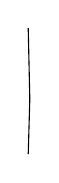
\begin{tikzpicture}\draw (0,0) -- (0.02,0.7) -- (0,1.6);\end{tikzpicture}}}}
\uline{Proposition}\handwritten{5.1.} Le foncteur $\mathbb{M}\handwritten{\longmapsto}V\otimes_{\underline{Z}_p}W$ est une équivalence de la catégorie des faisceaux $p$-adiques constructibles\handwritten{\,}sur $k$ vers la sous-catégorie pleine de la catégorie des F-cristaux \unsure{sur|sar} $k$, formée des F-cristaux $M$ tels que $F_M : M^{\handwritten{\sigma}}\handwritten{\longrightarrow}M$ soit un \uline{isomorphisme} .

\uline{Corollaire}\handwritten{5.\unsure{2|1}.} Le foncteur précédent induit un foncteur pleinement fidèle (compatible avec les $\otimes$-structures)\inserted{\handwritten{$i$}} de la catégorie des

\scanpage{72}
% archive sheet number: 71

$\underline{Q}_p$ faisceaux constructibles sur $k$ vers la catégorie $\mathrm{Fcriso}(k)$. Pour un objet \deleted{\unsure{$E$}}$(E,F_E)$ de cette dernière, les conditions suivantes sont équivalentes\inserted{(si $k$ parfait)}: a) $(E,F_E)$ appartient à l'image essentielle du foncteur précédent; b) il existe un réseau $M\subset E$ stable par $F_E$ \deleted{\unsure{sur}} \uline{et} par $F_E^{-1}$ (i.e. tel que $F_E$ induise un \uline{automorphisme} de $M$); c) la famille des i\handwritten{t}érés $F^{\unsure{m|n}}$, $n\quad\underline{Z}$, est bornée ; d) $E$ et $E^{\handwritten{\vee}}$ sont effectifs.

Les F-isocristaux en question sont appelés ``trivaux'' ou ``\uline{de pente nulle}''. On trouve ainsi un \uline{épimorphisme de gerbes}
\figure{\[
\underline{G}(k)\handwritten{\longrightarrow}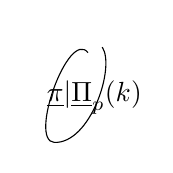
\begin{tikzpicture}[baseline=(gerbe.base)]
\node[inner sep=1pt] (gerbe) {$\handwritten{\unsure{\underline{\pi}|\underline{\Pi}}_{p}}(k)$};
\handwritten{\draw[thin] (-0.08,0.57) .. controls (-0.33,0.88) and (-0.84,-0.55) .. (-0.51,-0.57) .. controls (-0.05,-0.59) and (0.27,0.39) .. (0.10,0.64);}
\end{tikzpicture}\ ,
\]}
\margin{\handwritten{$\Pi$\par majuscule?}}
où $\handwritten{\underline{\pi}}_p(k)$ est la gerbe sur $\underline{Q}_p$ \deleted{des représentations continues} associée à la catégorie tannakienne des $\underline{Q}_p$-faisceaux constructibles, équivalente \deleted{à l'enveloppe alg} (une fois choisie une clôture algébrique $\bar{k}$ de $k$) à la gerbe triviale définie par l'enveloppe algébrique \deleted{du} $p$-adique du groupe pro-fini $\handwritten{\pi}=\operatorname{Gal}(\handwritten{\bar{k}}/k)$. Tenant compte de l'homomorphisme d'augmentation de \unsure{Gate|Tate}, on trouve même un homomorphisme
\[
\underline{G}(k)\handwritten{\longrightarrow\underline{\pi}}_p(k)\ \mathrm{x}\ \handwritten{[}\underline{G}_m\handwritten{]}_{\underline{Q}_p}
\]
où $\handwritten{[}\underline{G}_m\handwritten{]}$ est la gerbe triviale définie par $\underline{G}_m$ . On vérifie facilement que c'est encore un épimorphisme (i.e. que le foncteur
\[
(V_i)_{\handwritten{i}}\handwritten{\longmapsto\sum}V_i\otimes_{\underline{\mathbb{Q}}_p}\underline{Q}_p(i)
\]
allant de la catégorie des \deleted{\unsure{sh}} $\underline{Q}_p$-faisceaux constructibles \inserted{\handwritten{gradués}} sur $k$ vers $\mathrm{Fcriso}(k)$ est pleinement fidèle). Les F-isocristaux de la forme précédente pourraient être appelés les F-isocristaux \uline{de niveau zéro} .

\handwritten{6.} Considérons maintenant un \unsure{homomorphisme} de corps\deleted{x}
\[
k\handwritten{\longrightarrow}k'\ ,
\]
d'où un homomorphisme de catégories tannakiennes sur $\underline{Q}_p$
\[
\mathrm{Fcriso}(k)\handwritten{\longrightarrow}\mathrm{Fcriso}(\handwritten{k}')\ ,
\]
et un homomorphisme de gerbes tannakiennes sur $\underline{Q}_p$ en sens inverse

\scanpage{73}
% archive sheet number: 72

\[
\underline{G}(k')\handwritten{\longrightarrow}\underline{G}(k)\ .
\]
Ce dernier rend commutatif \inserted{(mod isomorphisme canonique)} le diagramme
\diagram{\begin{tikzcd}[ampersand replacement=\&,column sep=large,row sep=large]
\underline{G}(k\handwritten{'}) \handwritten{\arrow[r]} \handwritten{\arrow[d,dash,"{\unsure{\ }}" description]} \& \underline{G}(k^{\deleted{\unsure{'}}}) \handwritten{\arrow[d,dash,"{\unsure{\ }}" description]} \\
\handwritten{\unsure{\underline{\pi}|\underline{\Pi}}_{p}}(k')\mathrm{x}\handwritten{[}G_m\handwritten{]}_{\underline{\unsure{\mathbb{Q}|Q}}_p} \handwritten{\arrow[r]} \& \handwritten{\underline{\pi}}_p(k)\mathrm{x}\handwritten{[}\underline{G}_m\handwritten{]}_{\underline{Q}_p}
\end{tikzcd}}
(i.e. on a, sur les catégories tannakiennes\deleted{\unsure{, un}} correspondantes, un dia\unsure{g|gg}ramme comm\unsure{u|y}tatif à isomorphisme \inserted{can.} près).

Oubliant dans ce dernier les facteurs $\handwritten{[}\underline{G}_m\handwritten{]}$, on voit donc que $\underline{G}(k')\handwritten{\longrightarrow}\underline{G}(k)$ se factorise par la sous-\deleted{catégorie} gerbe de $\underline{G}(k)$ correspondant au sous-groupe fermé de $\handwritten{\pi}_1(k)$ image de $\handwritten{\pi}_1(k')$ ... A prouver:

\uline{Proposition} \handwritten{6.1.} Si $k'$ est une extension \deleted{finie} étale de $k$, alors l'homomorphisme de gerbes $\underline{G}(k')\handwritten{\longrightarrow}\underline{G}(k)$ est un \uline{monomorphisme} dont l'image est exactement la sous-gerbe ``ouverte'' définie ci-dessus. En particulier, si $k'$ est une extension finie galoisienne de $k$, \deleted{on a une} de groupe de Galois $g$, et on une suite exacte canonique de gerbes
\[
0\handwritten{\longrightarrow}\underset{\handwritten{\deleted{\unsure{\pi|\mu}}}}{\underline{G}^{\deleted{\unsure{'}}}}(k\handwritten{'})\handwritten{\longrightarrow}\underline{G}(k)\handwritten{\longrightarrow [}g\handwritten{]}_{\underline{Q}_p}\handwritten{\longrightarrow}0\ .
\]
Cet énoncé devrait être formellement équivalent au suivant: $\operatorname{Spec}(k')\handwritten{\longrightarrow}\operatorname{Spec}(k)$ est un morphisme de descente effective pour la catégorie fibrée des $\mathrm{Fcriso}(L)$ sur des composés finis\inserted{$L$} de corps de car. $p$. La démonstration de ce dernier fait est $\handwritten{\pm}$ triviale.

\uline{Question} \handwritten{6.2.} A-t-on encore un énoncé analogue lorsqu'on suppose que $k'$ est une extension galoisienne de $k$ qui peut-être infinie ? Le cas le plus intéressant serait celui où $k'$est la clôture séparable de $k$, de sorte qu'on aurait un dévissage de $\underline{G}(k)$ en
\[
0\handwritten{\longrightarrow}\underline{G}(\handwritten{\bar{k}}^{\deleted{\unsure{'}}})\handwritten{\longrightarrow}\underline{G}(k)\handwritten{\longrightarrow\underline{\pi}}_p(k)\handwritten{\longrightarrow}0\quad\deleted{\unsure{?}}\ ;
\tag*{\handwritten{(\unsure{6}.2.1)}}
\]
lorsque $k$ est parfait i.e. $\handwritten{\bar{k}}$ alg. clos, nous verrons que $\underline{G}(\handwritten{\bar{k}})$ ne dépend pas essentiellement de \handwritten{$k$. À}

\scanpage{74}
% archive sheet number: 73

\handwritten{7.} Nous verrons çi-dessus que la réponse à la question précédente est affirmative lorsque $k$ est un corps fini, en particulier si c'est le \unsure{corps|coops} premier $\underline{F}_p$, On trouve alors, grâce à cette structure d'extension sur $\underline{G}(\underline{F}_p)$, un homomorphisme canonique de Gerbes (pour tout $k$)
\[
\underline{G}(k)\handwritten{\simeq}\underline{G}(\underline{F}_p)\mathrm{x}_{\deleted{\unsure{\underline{G}(}}\handwritten{\unsure{\underline{\pi}|\underline{\Pi}}}_p(\underline{F}_p))}\handwritten{\underline{\pi}}_p(k)\ ,
\]
et pour $k$ parfait, une réponse affirmative à la question précédente revient à l'assertion que l'homomorphisme précédent est une équivalence de Gerbes. Comme on connait parfaitement bien la Gerbe $\underline{G}(\underline{F}_p)$ et son homomorphisme dans $\handwritten{\underline{\pi}}_p(\underline{F}_p)$ (cf plus bas) cela donnerait donc la structure de $\underline{G}(k)$ en termes de la connaiassance de \deleted{\unsure{$\pi_p(\underline{F}_p$}} $\handwritten{\underline{\pi}}_{\deleted{\unsure{a}}p}(k)$ (connu quand\handwritten{\,}on connait $\handwritten{\pi}_1(k)=\operatorname{Gal}(\handwritten{\bar{k}}/k)$) et \deleted{de} l'homomorphisme $\handwritten{\underline{\pi}}_p(k\deleted{\unsure{'}})\handwritten{\longrightarrow\underline{\pi}}_p(\underline{F}_p)$ (connu quand on connait $\handwritten{\pi}_1(k)\handwritten{\longrightarrow\pi}_1(\underline{F}_p)\handwritten{\longrightarrow}\handwritten{\hat{\underline{Z}}}$). Cela résoudrait donc la question de la structure de $\underline{G}(k)$ pour $k$ parfait. On notera que l'objet de Tate de $\mathrm{Fc}\handwritten{\mathrm{r}}\mathrm{iso}(k)$ provient de celui de $\mathrm{Fcriso}(\underline{F}_p)$ et sera donc également déterminé. Le foncteur fibre canonique sur $K$\inserted{$=K(k)$} correspond alors à un foncteur fibre de $\mathrm{Fcriso}(\underline{F}_p)$ sur $K$, un foncteur fibre de \deleted{\unsure{$\underline{\pi}_p(k)$}}\inserted{la catégorie des $\underline{Q}_p$-faisceaux constr. sur $k$} sur $K$, et un isomorphisme entre les ``restrictions'' de ces foncteurs à la catégorie des $\underline{Q}_p$-faisceaux constructibles sur $\underline{F}_p$ ; or le premier foncteur fibre n'est autre que \inserted{celui déduit par} l'extension des scalaires $\underline{Q}_p=K\handwritten{(}\underline{F}_p)\handwritten{\longrightarrow}K=K(k)$ du foncteur fibre analogue sur $\unsure{\mathbb{F}|\mathrm{F}|\mathrm{G}}\mathrm{criso}(\underline{F}_p)$, le deuxième est \unsure{le|he} foncteur \inserted{\handwritten{$i$:}} $V\handwritten{\mapsto}V\otimes_{\underline{Q}_p}K$, et l'isomorphisme \deleted{canonique} entre les restrictions est l'isomorphisme canonique évident\inserted{\handwritten{(compatibilité de $i$ aux changements de corps de base)}}. Donc la structure supplémentaire de $\underline{G}(k)$ (savoir sa section \deleted{sur} canonique sur $K$) est déterminée par la connaissance de la section de $\handwritten{\underline{\pi}}_p(k)$ sur $K$ (i.e. le foncteur précédent $V\handwritten{\mapsto}V\otimes_{\underline{Q}_p}K$ ) et l'isomorphisme de l'\unsure{image|iamge} de ladite section dans $\handwritten{\underline{\pi}}_p(\underline{F}_p)$ avec la section provenant de\deleted{\unsure{s}} la section canonique de $\handwritten{\underline{\pi}}_p(\underline{F}_p)$ sur $\underline{Q}_p$ ; ce sont là des données qui ne sont évidemment pas contenues dans celle du groupe

\margin{\handwritten{\uline{NB} On a donc, en comparant le foncteur ``fibre \deleted{``\unsure{oubli}} en $\bar{k}$'' sur $Q_p$, et le foncteur précédent, un torseur canonique sur $K$ de groupe \deleted{\unsure{de}}\unsure{lien} $\underline{\pi}_p(k)_K$\deleted{\illegible{2} $\unsure{Q_p|\mathbb{Q}_p}$}}}

\scanpage{75}
% archive sheet number: 74

\margin{\handwritten{On a un hom (une fois choisi $\bar{k}$ ; d'où une réalisation \deleted{\unsure{$G'|C'$}} de lien $\unsure{\underline{\pi}|\underline{\Pi}}_p(k)$) $\pi_1(k)_K\longrightarrow\unsure{G'|C'}(K)$ d'où un foncteur $(\text{torseurs sous }\pi_1(k)_K)\longrightarrow\text{torseurs sous }G'$ \unsure{Et|et} on prend l'image du torseur sous $\pi_1(k)_K$, défini en interprétant $\pi_1(k)$ comme Galois de l'extension non ramifiée \unsure{universelle} de $K$.}}
pro-fini ``abstrait'' $\handwritten{\pi}_1(k)$, mais on se convainc facilement qu'elles\deleted{\unsure{sont}} sont contenues dans la donnée de ce groupe, $+$ son opération sur la clôture algébrique $\handwritten{\bar{K}}$ de $K$ (ou simplement, sur sa clôture non ramifiée .sur $W$ ...)\handwritten{/}. - Il resterait enfin à déterminer la structure d'effectivité dans la catégorie $\mathrm{Fcriso}(k)$ dé\deleted{\unsure{terminé}}\handwritten{\unsure{terminé}}e par la récette précédente\deleted{\unsure{.} la suggestion naturelle est que $\mathrm{Fcriso}^{\handwritten{+}}(k)$ est engendré par les images de $\mathrm{Fcriso}^{\handwritten{+}}$} Or il est immédiat que l'effectivité d'un \unsure{F-isocrristal|F-isocristal} est invariante par changement de base, en particulier par le changement de base $k\handwritten{\longrightarrow\bar{k}}$, ce qui ramène au cas d'un $k$ algébriquement clos, ou encore au cas de $\underline{F}_p$ . \deleted{En}\handwritten{Dans} \deleted{termes de} la terminologie introduite plus bas, on trouvera donc que les $\unsure{\mathbb{F}|F|E}$-isocristaux effectifs sont ceux qui sont \uline{à pente} $\handwritten{\geq}0$ (i.e. dont toutes les composantes isopentiques \deleted{sont} non nulles sont de pente $\handwritten{>}\ 0$).

\handwritten{8.} Il reste donc à étudier la gerbe $\underline{G}(\underline{F}_p)$, avec s\deleted{\unsure{on}}a \deleted{foncteur fibre} section canonique sur $\underline{Q}_p$, sa structure d'extension, et sa structure d'effectivité.

\margin{\handwritten{\figure{\begin{tikzpicture}\draw (0,0) -- (0.65,0.04) -- (0.65,0.8) -- (1.1,0.8);\end{tikzpicture}}}}
\inserted{\handwritten{8.1.}} Tout d'abord, la donnée du foncteur fibre canonique permet d'identifier $\underline{G}(\underline{F}_p)$ à la gerbe\handwritten{\,}triviale définie par le lien \inserted{\handwritten{$G$}} de cette gerbe. Comme $\mathrm{Fcriso}(F_p)$ avec son foncteur fibre s'identifie à la catégorie des automorphismesde\inserted{$F_E$} vectoriels de dimension finie\inserted{$E$} sur $\underline{Q}_p$, avec le foncteur ``oubli de $F_E$ '', on voit que le lien de la gerbe est l'enveloppe $\underline{Q}_p$-\inserted{pro}algébrique de groupe discret $\underline{Z}$ . Soit $G$ ce groupe affine sur $\underline{Q}_p$ . I\handwritten{l} est évidemment commutatif, donc produit d'un groupe vectoriel $G_u$ par un groupe de t.m. $G_{\deleted{\unsure{m}}r}$ .
\margin{\handwritten{\unsure{réf}\figure{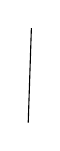
\begin{tikzpicture}\draw (0,0) -- (0.04,1.2);\end{tikzpicture}}}}
Ce dernier est l'enveloppe \inserted{de type} multiplicati\deleted{ve}\handwritten{f} du groupe $\underline{Z}$, et il s'ensuit aussitôt que c'est le groupe de t.m. dont le groupe des caractères sur $\handwritten{\bar{\underline{Q}}}_p$ est donné par
\[
\handwritten{\Gamma}=\handwritten{\bar{\underline{Q}}}_p^{\handwritten{*}}\ ,
\]
\handwritten{(}isomorphisme compatible avec l'action de $\operatorname{Gal}(\handwritten{\bar{\underline{Q}}}_p/\underline{Q}_p)$ ). D'autre

\scanpage{76}
% archive sheet number: 75

part, \inserted{\handwritten{\uline{une fois choisi} \uline{une clôture} $\overline{\mathbb{F}}_p$,}} la gerbe $\handwritten{\unsure{\underline{\pi}|\underline{\Pi}}}_p(\underline{F}_p)$, grâce àu\deleted{son} foncteur \unsure{fvbre|fibre|fïbre} évident ``fibre en $\handwritten{\bar{\underline{F}}}_p$ '' sur la catégorie des $\underline{Q}_p$-faisceaux constructibles sur $\underline{F}_p$, s'identifie à la \deleted{catégorie}\inserted{gerbe triviale définie\deleted{\unsure{et}} par l'}enveloppe $\underline{Q}_p$-\unsure{algébriqueque|algébrique} du groupe profini $\handwritten{\pi}_1(\underline{F}_p)=\handwritten{\bar{\underline{Z}}}\deleted{\unsure{r}}$, \deleted{lequel, comme on le constate aisément, est le}

Un \inserted{$\underline{Q}_p$-}faisceau constructible sur $\underline{F}_p$ s'identifie à un vectoriel de dimension finie $E$ sur $\underline{Q}_p$, muni d'un automorphisme $F_E$ tel que l'\deleted{hom} opération $n\handwritten{\mapsto}F_E^n$ de $\underline{Z}$ sur $E$ se prolonge par continuité en une opération de \deleted{\unsure{$\hat{\underline{Z}}$}} $\handwritten{\hat{\underline{Z}}}$ \margin{\handwritten{$Z$}}. Identifiant \inserted{\handwritten{(par un foncteur $j$, \uline{distinct} de celui de 5.2)}} la catégorie de ces $(E,\deleted{\unsure{E_E}}F_E)$ à une\handwritten{\,}sous-catégorie pleine de\deleted{\unsure{s}} la catégorie \deleted{des} $\mathrm{Fcriso}(\underline{Q}_p)$ des couples $(E,F_E)$, où $F_E$ est un automorphisme \uline{quelconque}, on voit que le lien \deleted{de notre}\inserted{$G\handwritten{'}$ de} $\handwritten{\underline{\pi}}_p(\underline{F}_p)$ de cette catégorie s'identifie à un quotient du lien $G$ de $\mathrm{Fcriso}(\underline{F}_p)$ déterminé plus haut, et on voit aussitôt que ce quotient est de la forme $G_u\mathrm{x}G_r^{\deleted{\unsure{x}}\handwritten{'}}$, où $G_r'$ est \unsure{le|he} qutient de $G_r$ (ceci revient à dire que si on décompose $F_E$ en produit de sa composante unipotente par sa composante semi-simple, alors la condition que $F_E$ définisse une opération de $\handwritten{\hat{\underline{Z}}}$ ne dépend que de la composante semi-simple); de façon précise, $G'_r$ est le groupe quotient de $G_r$ défini par le sous-groupe du groupe des caractères $\handwritten{\bar{\underline{Q}}}_p^{\handwritten{*}}$ de $G_r$ formé des \uline{unités} p\uline{\unsure{éadiques|-adiques}} : cela signifie en effet que $F_E$ définit uneopération de \deleted{\unsure{$F_E$}} $\handwritten{\hat{\underline{Z}}}$ (i.e. définit un F-isocristal de pente nulle) sss les valeurs\deleted{\unsure{s}} propres de $F_E$ sont des unités, ce qui résulte en effet aussitôt du critère donné plus haut des F-isocristaux de pente nulle (ou se vérifie directement de façon immédiate; la référence au résultat sur les fourbis de pente nulle devrait se justifier par un grain de sel, car l'inclusion utilisée ici des $\underline{Q}_p$-faisceaux constructibles sur $\underline{F}_p$ dans\deleted{\unsure{à}} les F-iso\deleted{\unsure{cr}}cristaux n'est pas celle utilisée \deleted{plus haut}\inserted{\handwritten{dans 5.2}}, cf. plus bas). On trouve ainsi une structure d'extension sur $G\handwritten{=}\operatorname{Lien}(\underline{G}(\underline{F}_p))$:
\[
0\handwritten{\longrightarrow}H\handwritten{\longrightarrow}G\handwritten{\longrightarrow}G'\handwritten{\longrightarrow}0\ ,
\]
où $H$ est le groupe de t.m. dont le groupe des caractères est le

